\documentclass{../khlslides}

\usetikzlibrary{arrows.meta}

\title[Arrays]{Arrays}
\author{Fr\'ed\'eric Vogels}



\newcommand{\drawarray}[1]{
  \foreach[count=\i] \val in {#1} {
    \pgfmathparse{int(\i-1)}\let\idx\pgfmathresult
    \pgfmathparse{(\i-1)*1.2}\let\x\pgfmathresult
    \node[anchor=south west,cell] (cell \i) at (\x, 0) {\val};
    \node[index] at (cell \i.north west) {\tiny\idx};
  }
}

\newcommand{\drawheterogeneousarray}[1]{
  \foreach[count=\i] \val/\cell in {#1} {
    \pgfmathparse{int(\i-1)}\let\idx\pgfmathresult
    \pgfmathparse{(\i-1)*1.2}\let\x\pgfmathresult
    \node[anchor=south west,\cell] (cell \i) at (\x, 0) {\val};
    \node[index] at (cell \i.north west) {\tiny\idx};
  }
}

\pgfkeys{/tikz/.cd,
         cell/.style={drop shadow,fill=blue!50,minimum size=.8cm},
         cell/.style={drop shadow,fill=blue!50,minimum size=.8cm},
         highlighted cell/.style={drop shadow,fill=green!50,minimum size=.8cm},
         index/.style={fill=white,draw},
         box/.style={fill=red!10,drop shadow}}


\begin{document}

\begin{frame}
  \titlepage
\end{frame}


\begin{frame}
  \frametitle{Probleem: Gelukkige Getallen (VPW2011)}
  \begin{center} \large\bfseries
    De \emph{opvolger} van een getal is de som van zijn cijfers.
  \end{center}
  \vskip4mm
  \[
    \begin{array}{r@{}c@{}lcccccc}
      \mathrm{opvolger}(&11&) & = & 1^2 + 1^2 & = & 1 + 1 & = & 2 \\
      \mathrm{opvolger}(&49&) & = & 4^2 + 9^2 & = & 16 + 81 & = & 97 \\
      \mathrm{opvolger}(&123&) & = & 1^2 + 2^2 + 3^2 & = & 1 + 4 + 9 & = & 14
    \end{array}
  \]
\end{frame}

\begin{frame}
  \frametitle{Probleem: Gelukkige Getallen (VPW2011)}
  \begin{center}
    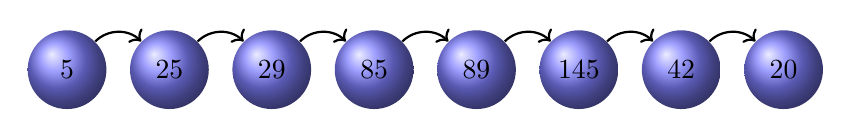
\begin{tikzpicture}[node/.style={ball color=blue!50,circle,minimum size=1cm}]
      \foreach[count=\i] \c in {5,25,29,85,89,145,42,20} {
        \pgfmathparse{\i*1.3}\let\cx\pgfmathresult
        \node[node] (node \i) at (\cx,0) {\c};
      }
      \foreach \i in {1,...,7} {
        \pgfmathparse{int(\i+1)}\let\j\pgfmathresult
        \draw[->,thick] (node \i.north east) to [bend left=45] (node \j.north west);
      }
    \end{tikzpicture}
  \end{center}
  \vskip5mm
  \begin{center}
    \large Ketting van opvolgers
  \end{center}    
\end{frame}

\begin{frame}
  \frametitle{Probleem: Gelukkige Getallen (VPW2011)}
  \begin{center} \Large\bfseries
    \emph{Gelukkig getal}: ketting eindigt op 1.
  \end{center}

  \begin{columns}
    \column{.5\linewidth}
    \begin{center}
      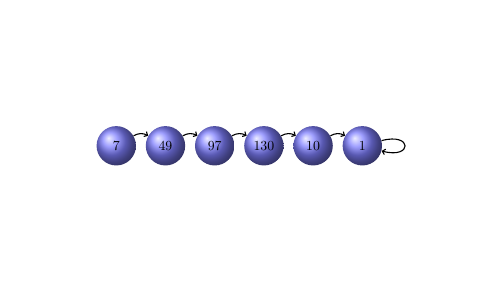
\begin{tikzpicture}[transform shape,scale=0.5,
                          node/.style={ball color=blue!50,circle,minimum size=1cm},
                          arrow/.style={-{Straight Barb[length=1pt]}}]
        \path[use as bounding box] (-1,-3) rectangle (10,3);
        \foreach[count=\i] \c in {7,49,97,130,10,1} { 
          \pgfmathparse{\i*1.25}\let\x\pgfmathresult
          \node[node] (node \i) at (\x,0) {\c};
        }

        \foreach \i in {1,...,5} {
          \pgfmathparse{int(\i+1)}\let\j\pgfmathresult
          \draw[arrow] (node \i) to [bend left=30] (node \j);
        }
        \draw[arrow] (node 6) to [loop right] (node 6);
      \end{tikzpicture}
    \end{center}
    \begin{center} 7 is gelukkig \end{center}

    \column{.5\linewidth}
    \begin{center}
      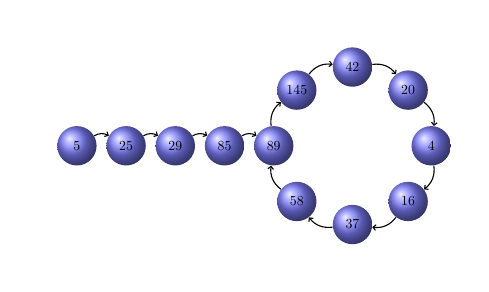
\begin{tikzpicture}[transform shape,scale=0.5,
                          node/.style={ball color=blue!50,circle,minimum size=1cm},
                          arrow/.style={-{Straight Barb[length=1pt]}}]
        \path[use as bounding box] (0,-3) rectangle (11,3);

        \foreach[count=\i] \c in {5,25,29,85} { 
          \pgfmathparse{\i*1.25}\let\x\pgfmathresult
          \node[node] (node \i) at (\x,0) {\c};
        }
        \foreach[count=\i] \c in {89,145,42,20,4,16,37,58} {
          \pgfmathparse{int(\i+4)}\let\j\pgfmathresult
          \pgfmathparse{180-360/8*(\i-1)}\let\angle\pgfmathresult
          \node[node,xshift=8.25cm] (node \j) at (\angle:2cm) {\c};
        }
        \foreach \i in {1,...,11} {
          \pgfmathparse{int(\i+1)}\let\j\pgfmathresult
          \draw[arrow] (node \i) to [bend left=30] (node \j);
        }
        \draw[arrow] (node 12) to [bend left=30] (node 5);
      \end{tikzpicture}
    \end{center}
    \begin{center} 5 is ongelukkig \end{center}
  \end{columns}
\end{frame}

\begin{frame}
  \frametitle{Probleem: Gelukkige Getallen (VPW2011)}
  \begin{center} \Large
    Opgave: schrijf een functie {\tt gelukkig(n)} die nagaat
    of {\tt n} gelukkig is.
  \end{center}
\end{frame}

\begin{frame}
  \frametitle{Eerste poging}
  \code[width=.6\linewidth]{first-attempt.js}
  \visible<2>{
    \begin{center}
      Kan geen ongelukkige getallen detecteren: oneindige lus.
    \end{center}
  }
\end{frame}

{
\newcommand{\drawgraph}[1]{{
  \let\activenode#1
  \foreach[count=\i] \c in {5,25,29,85} { 
    \pgfmathparse{\i*1.25}\let\x\pgfmathresult
    \pgfmathparse{ifthenelse(equal(\i,\activenode),"selected node","node")}\let\s\pgfmathresult
    \node[\s] (node \i) at (\x,0) {\c};
  }
  \foreach[count=\i] \c in {89,145,42,20,4,16,37,58} {
    \pgfmathparse{int(\i+4)}\let\j\pgfmathresult
    \pgfmathparse{180-360/8*(\i-1)}\let\angle\pgfmathresult
    \pgfmathparse{ifthenelse(equal(\j,\activenode),"selected node","node")}\let\s\pgfmathresult
    \node[\s,xshift=8.25cm] (node \j) at (\angle:2cm) {\c};
  }
  \foreach \i in {1,...,11} {
    \pgfmathparse{int(\i+1)}\let\j\pgfmathresult
    \draw[arrow] (node \i) to [bend left=30] (node \j);
  }
  \draw[arrow] (node 12) to [bend left=30] (node 5);
}}

\begin{frame}
  \begin{center}
    \begin{tikzpicture}[node/.style={ball color=blue!50,circle,minimum size=1cm},
                        selected node/.style={node,ball color=green!50},
                        arrow/.style={-latex}]
      \foreach[count=\slideindex] \i in {1,...,12,5,6,...,12} {
        \only<\slideindex>{
          \drawgraph{\i}
        }
      }
    \end{tikzpicture}
  \end{center}
\end{frame}
}

\begin{frame}
  \begin{center} \Large
    Hoe lossen we dit best op?
  \end{center}
\end{frame}

{
\newcommand{\drawgraph}[1]{{
  \let\activenode#1
  \foreach[count=\i] \c in {5,25,29,85} { 
    \pgfmathparse{\i*1.25}\let\x\pgfmathresult
    \pgfmathparse{ifthenelse(\i<\activenode,"visited node",ifthenelse(equal(\i,\activenode),"selected node", "node"))}\let\s\pgfmathresult
    \node[\s] (node \i) at (\x,0) {\c};
  }
  \foreach[count=\i] \c in {89,145,42,20,4,16,37,58} {
    \pgfmathparse{int(\i+4)}\let\j\pgfmathresult
    \pgfmathparse{180-360/8*(\i-1)}\let\angle\pgfmathresult
    \pgfmathparse{ifthenelse(\j<\activenode,"visited node",ifthenelse(equal(\j,\activenode),"selected node", "node"))}\let\s\pgfmathresult
    \node[\s,xshift=8.25cm] (node \j) at (\angle:2cm) {\c};
  }
  \foreach \i in {1,...,11} {
    \pgfmathparse{int(\i+1)}\let\j\pgfmathresult
    \draw[arrow] (node \i) to [bend left=30] (node \j);
  }
  \draw[arrow] (node 12) to [bend left=30] (node 5);
}}

\begin{frame}
  \begin{center}
    \begin{tikzpicture}[node/.style={ball color=blue!50,circle,minimum size=1cm},
                        selected node/.style={node,ball color=green!50},
                        visited node/.style={node,ball color=red!50},
                        arrow/.style={-latex}]
      \foreach[count=\slideindex] \i in {1,...,12} {
        \only<\slideindex>{
          \drawgraph{\i}
        }
      }
    \end{tikzpicture}
  \end{center}
\end{frame}
}

\begin{frame}
  \frametitle{Gebruik makend van verzamelingen}
  \code[width=.9\linewidth]{with-set.js}
\end{frame}


%%% Local Variables: 
%%% mode: latex
%%% TeX-master: "slides"
%%% End: 

% {
  \newcommand{\CODE}[1]{
    \onslide<#1>
    \begin{minipage}[c][2cm]{\linewidth}
      \code[width=.8\linewidth]{array-basics-#1.js}
    \end{minipage}
  }
  \newcommand{\ARRAY}[2]{
    \only<#1>{\drawarray{#2}}
  }

  \begin{frame}
    \frametitle{Arrays}
    \begin{center}
      \begin{tikzpicture}
        \coordinate (lower left) at (-.5,-.5);
        \coordinate (upper right) at (6,1.5);
        \coordinate (upper left) at (lower left |- upper right);
        \coordinate (lower right) at (lower left -| upper right);

        \draw[use as bounding box,box] (lower left) rectangle (upper right);
        \node[anchor=south] at ($ (upper left) !.5! (upper right) $) {\sc \Large \color{gray} voor};
        \ARRAY{2}{,,,,}
        \ARRAY{3}{5,,,,}
        \ARRAY{4}{5,4,,,}
        \ARRAY{5}{5,4,5,,}
        \ARRAY{6}{5,4,5,4,}
      \end{tikzpicture}
    \end{center}

    \begin{overprint}
      \CODE{1}
      \CODE{2}
      \CODE{3}
      \CODE{4}
      \CODE{5}
      \CODE{6}
    \end{overprint}

    \begin{center}
      \begin{tikzpicture}
        \coordinate (lower left) at (-.5,-.5);
        \coordinate (upper right) at (6,1.5);
        \coordinate (upper left) at (lower left |- upper right);
        \coordinate (lower right) at (lower left -| upper right);

        \draw[use as bounding box,box] (lower left) rectangle (upper right);
        \node[anchor=north] at ($ (lower left) !.5! (lower right) $) {\sc \Large \color{gray} na};
        \ARRAY{1}{,,,,}
        \ARRAY{2}{5,,,,}
        \ARRAY{3}{5,4,,,}
        \ARRAY{4}{5,4,5,,}
        \ARRAY{5}{5,4,5,4,}
        \ARRAY{6}{5,4,5,4,18}
      \end{tikzpicture}
    \end{center}
  \end{frame}
}

\begin{frame}
  \frametitle{Itereren over Array}
  \vskip1cm
  \code[width=.95\linewidth]{iteration.js}
  \begin{tikzpicture}[overlay,remember picture]
    \only<2>{
      \node[/khl/note,anchor=south] (note init) at ($ (init) + (0,1) $) {
        \parbox{5cm}{
          Eerste element heeft index 0.
        }
      };
      \draw[/khl/note arrow] (note init) -- (init);
    }
    \only<3>{
      \node[/khl/note,anchor=south] (note cond) at ($ (cond) + (0,1) $) {
        \parbox{7cm}{
          Index moet gaan van 0 t.e.m.\ {\tt length-1}!
        }
      };
      \draw[/khl/note arrow] (note cond) -- (cond);
    }
  \end{tikzpicture}

  \visible<3>{
    \begin{center}
      \begin{tikzpicture}
        \drawarray{,,,,}
        \draw[|-|] ($ (cell 1.south west) + (0,-.2) $) -- ($ (cell 5.south east) + (0,-.2) $)
          node[midway,below] {lengte 5};
      \end{tikzpicture}
    \end{center}   
  }
\end{frame}

\begin{frame}
  \frametitle{Oefening}
  \begin{center} \Large
    Schrijf een functie {\tt verdubbel} die een array ontvangt en elk element ervan verdubbelt.
  \end{center}
  \vskip4mm
  \code[width=.95\linewidth]{iteration.js}
\end{frame}

\begin{frame}
  \frametitle{Oplossing}
  \code[width=.95\linewidth]{double.js}
\end{frame}


{
  \pgfkeys{/tikz/.cd,
           cell/.style={drop shadow,fill=blue!50,minimum size=.8cm},
           index/.style={fill=white,draw},
           box/.style={fill=red!10,drop shadow}}
  \newcommand{\CODE}[1]{
    \onslide<#1>
    \begin{minipage}[c][2cm]{\linewidth}
      \code{array-advanced-#1.js}
    \end{minipage}
  }
  \newcommand{\ARRAY}[2]{
    \only<#1>{\drawarray{#2}}
  }

  \begin{frame}
    \frametitle{Array Modification}
    \begin{center}
      \begin{tikzpicture}
        \coordinate (lower left) at (-.5,-.5);
        \coordinate (upper right) at (6,1.5);
        \coordinate (upper left) at (lower left |- upper right);
        \coordinate (lower right) at (lower left -| upper right);

        \draw[use as bounding box,box] (lower left) rectangle (upper right);
        \node[anchor=south] at ($ (upper left) !.5! (upper right) $) {\sc \Large \color{gray} voor};
        \ARRAY{2}{1,2,3}
        \ARRAY{3}{1,2,3,4}
        \ARRAY{4}{1,2,3}
        \ARRAY{5}{0,1,2,3}
      \end{tikzpicture}
    \end{center}

    \begin{overprint}
      \CODE{1}
      \CODE{2}
      \CODE{3}
      \CODE{4}
      \CODE{5}
    \end{overprint}

    \begin{center}
      \begin{tikzpicture}
        \coordinate (lower left) at (-.5,-.5);
        \coordinate (upper right) at (6,1.5);
        \coordinate (upper left) at (lower left |- upper right);
        \coordinate (lower right) at (lower left -| upper right);

        \draw[use as bounding box,box] (lower left) rectangle (upper right);
        \node[anchor=north] at ($ (lower left) !.5! (lower right) $) {\sc \Large \color{gray} na};
        \ARRAY{1}{1,2,3}
        \ARRAY{2}{1,2,3,4}
        \ARRAY{3}{1,2,3}
        \ARRAY{4}{0,1,2,3}
        \ARRAY{5}{1,2,3}
      \end{tikzpicture}
    \end{center}
  \end{frame}
}

\begin{frame}
  \frametitle{Array Modification}
  \begin{center}
    \begin{tikzpicture}
      \drawarray{1,2,3,4,5}
      \coordinate (position extra left) at ($ (cell 1.south west) + (-1.2,0) $);
      \coordinate (position extra right) at ($ (cell 5.south west) + (1.2,0) $);
      \node[minimum size=.8cm,draw,dashed,anchor=south west] (extra left) at (position extra left) {};
      \node[minimum size=.8cm,draw,dashed,anchor=south west] (extra right) at (position extra right) {};
      \draw[->] (extra left.north) +(1,1) .. controls +(left:.5cm) and +(up:.5cm) .. +(0,0) node[midway,sloped,above] {\tiny unshift};
      \draw[->] (extra left.south) .. controls +(down:.5cm) and +(left:.5cm) .. +(1,-1) node[midway,sloped,below] {\tiny shift};
      \draw[->] (extra right.north) +(-1,1) .. controls +(right:.5cm) and +(up:.5cm) .. +(0,0) node[midway,sloped,above] {\tiny push};
      \draw[->] (extra right.south) .. controls +(down:.5cm) and +(right:.5cm) .. +(-1,-1) node[midway,sloped,below] {\tiny pop};
    \end{tikzpicture}
  \end{center}
\end{frame}

{
\pgfkeys{/tikz/.cd,
         cell/.style={drop shadow,fill=blue!50,minimum size=.8cm},
         index/.style={fill=white,draw},
         box/.style={fill=red!10,drop shadow}}
\newcommand{\CODE}[1]{
  \onslide<#1>
  \begin{minipage}[c][1cm]{\linewidth}
    \code{array-slice-#1.js}
  \end{minipage}
}
\newcommand{\ARRAY}[2]{
  \only<#1>{\drawarray{#2}}
}

\begin{frame}
  \frametitle{Arrays Slicing}
  \begin{center}
    \begin{tikzpicture}
      \coordinate (lower left) at (-.5,-.5);
      \coordinate (upper right) at (6,1.5);
      \coordinate (upper left) at (lower left |- upper right);
      \coordinate (lower right) at (lower left -| upper right);

      \draw[use as bounding box,box] (lower left) rectangle (upper right);
      \node[anchor=south] at ($ (upper left) !.5! (upper right) $) {\sc \Large \color{gray} voor};
      \ARRAY{1-}{1,2,3,4,5}
      \node (xs) at ($ (cell 1.west) + (-1,0) $) {xs};
      \draw[->] (xs) to (cell 1.west);
    \end{tikzpicture}
  \end{center}

  \begin{overprint}
    \CODE{1}
    \CODE{2}
    \CODE{3}
  \end{overprint}

  \begin{center}
    \begin{tikzpicture}
      \coordinate (lower left) at (-.5,-1.5);
      \coordinate (upper right) at (6,1.5);
      \coordinate (upper left) at (lower left |- upper right);
      \coordinate (lower right) at (lower left -| upper right);

      \draw[use as bounding box,box] (lower left) rectangle (upper right);
      \node[anchor=north] at ($ (lower left) !.5! (lower right) $) {\sc \Large \color{gray} na};
      \begin{scope}[yshift=.25cm]
        \ARRAY{1-}{1,2,3,4,5}
        \node (xs) at ($ (cell 1.west) + (-1,0) $) {xs};
        \draw[->] (xs) to (cell 1.west);
      \end{scope}
      \begin{scope}[yshift=-1.25cm]
        \ARRAY{1}{2,3,4}
        \ARRAY{2}{0,1}
        \ARRAY{3}{3,4,5}
        \node (ys) at ($ (cell 1.west) + (-1,0) $) {ys};
        \draw[->] (ys) to (cell 1.west);
      \end{scope}
    \end{tikzpicture}
  \end{center}
\end{frame}
}


\begin{frame}
  \frametitle{Array Concatenation}
  \begin{center}
    \begin{tikzpicture}[scale=.9,transform shape]
      \coordinate (lower left) at (-.5,-1);
      \coordinate (upper right) at (6,1.5);
      \coordinate (upper left) at (lower left |- upper right);
      \coordinate (lower right) at (lower left -| upper right);

      \draw[use as bounding box,box] (lower left) rectangle (upper right);
      \node[anchor=south] at ($ (upper left) !.5! (upper right) $) {\sc \Large \color{gray} voor};

      \begin{scope}[yshift=.25cm]
        \drawarray{1,2,3}
        \node (xs) at ($ (cell 1.west) + (-1,0) $) {xs};
        \draw[->] (xs) to (cell 1.west);
      \end{scope}
      \begin{scope}[yshift=-.75cm]
        \drawarray{4,5}
        \node (ys) at ($ (cell 1.west) + (-1,0) $) {ys};
        \draw[->] (ys) to (cell 1.west);
      \end{scope}
    \end{tikzpicture}
  \end{center}

  \code{concat.js}

  \begin{center}
    \begin{tikzpicture}[scale=.9,transform shape]
      \coordinate (lower left) at (-.5,-2.5);
      \coordinate (upper right) at (6,1.5);
      \coordinate (upper left) at (lower left |- upper right);
      \coordinate (lower right) at (lower left -| upper right);

      \draw[use as bounding box,box] (lower left) rectangle (upper right);
      \node[anchor=north] at ($ (lower left) !.5! (lower right) $) {\sc \Large \color{gray} na};
      \begin{scope}[yshift=.25cm]
        \drawarray{1,2,3}
        \node (xs) at ($ (cell 1.west) + (-1,0) $) {xs};
        \draw[->] (xs) to (cell 1.west);
      \end{scope}
      \begin{scope}[yshift=-1cm]
        \drawarray{4,5}
        \node (ys) at ($ (cell 1.west) + (-1,0) $) {ys};
        \draw[->] (ys) to (cell 1.west);
      \end{scope}
      \begin{scope}[yshift=-2.25cm]
        \drawarray{1,2,3,4,5}
        \node (zs) at ($ (cell 1.west) + (-1,0) $) {zs};
        \draw[->] (zs) to (cell 1.west);
      \end{scope}
    \end{tikzpicture}
  \end{center}
\end{frame}




%%% Local Variables: 
%%% mode: latex
%%% TeX-master: "arrays"
%%% End: 



\end{document}



%%% Local Variables: 
%%% mode: latex
%%% TeX-master: t
%%% End: 
